\chapter{Survey on Visualization Tools and Applications}
\label{ch:ch4}

\begin{flushright}
\textit{``I think we have consensus, RDF is something \\
you don't show your end users.''\footnote{\url{https://twitter.com/philarcher1/status/507856407127814145}}}  \\
Phil Archer (W3C Data Activity Lead)
\end{flushright}


\textcolor{red}{Content: 
 Tools for visualizations: facete, soA, etc.
 Survey on visualizations applications
 Explore limitations
 Find answers
\end{itemize}}

\section{Introduction}
\label{sec:intro-ch4}


According to \cite{marti2009} the main goal of information visualization is to translate abstract information into a visual form that provides new insight about that information, in a clearly and precise form. Data classification, either quantitative or categorical, is useful for the purpose of visualization, and can make differences between tools. Hierarchical faceted metadata is used to build a set of category hierarchies where each dimension is relevant to the collection for navigation. The resulting interface is known as faceted navigation, or guided navigation \cite{hearst02}. 
We have surveyed a number of visualization tools - fifteen to be precise- used to build applications over data in general (raw or structured) based on the following features:
\begin{itemize}
\item \textit{Data Formats} for the format of data taken as input by the tool;
\item \textit{Data Access}, for the way to access the data from the tool, such as web service, sparql endpoint, etc.
\item \textit{Language code}, the programming language used to develop the tool;
\item \textit{Type of Views}, the different views potentially accessible when using the tool;
\item \textit{Imported Libraries}, the external libraries available within the tool,
\item \textit{License} for the Intellectual Properties rights of the tool,
\item \textit{SemWeb Compliant}, whether the tool can be easily transposed or compliant with structured data; and 
\item \textit{Creator}, organizations or persons who developed the tool.

\end{itemize}
\todo{ADD Visual Box in the survey of Table \ref{tab:visuTools} }

\section{Tools for visualizing Structured Data}
\label{sec:strucdataviz}
In this section, we describe also visualization tools that natively do not take as input RDF data for two reasons: 
\begin{itemize}
\item those tools are relatively ``popular'' for analyzing data exposed by the government and agencies  (most of them in XLS, CSV) as they quickly make it easy to the users  to build chart  maps and compare with other datasets. One widely application is in the data journalism  where facts are analyzed by those tools without waiting for the semantic publication of the data 
\item Also these tools have many options for visualizing data and are not totally adapted in the Semantic Web community.

\end{itemize}

\subsection{Choosel}
\label{sec:choosel}

\texttt{Choosel} \cite{lars2010} is built on top of GWT  and the Google App Engine  (the backend can be modified to run on any servlet container). The client-side framework facilitates the interaction with visualization components, which can be wrappers around third party components and toolkits such as the Simile Timeline, Protovis and FlexViz. Choosel can integrate components developed using different technologies such as Flash and JavaScript. It is possible to implement visualization components that are compatible with the Choosel visualization component API. These visualization components can then be used to take advantage of Choosel features such as management of view synchronization, management of selections, and support for hovering and details on demand.

\subsection{Many Eyes}
\label{sec:manyEyes}
\texttt{Many Eyes} \cite{ibm2010} is a website that provides means to visualize data such as numbers, text and geographic information. It provides a range of visualizations including unusual ones such as ``treemaps''  and ``phrase trees''. All the charts made in Many Eyes are interactive, so it is possible to change what data is shown and how it is displayed. Many Eyes is also an online community where users can create groups (such as ``Ebola Crisis'' or ``Kobane War'') to organize, share and discuss data visualizations. Users can also comment on visualizations made by others, which is a good way to improve their work. The authors claim that it is useful because it users can build quick and easily visualizations from their own data, with the possibility to share them. is quick and easy to make and share great looking and fun to use visualizations from your own data. Data input formats are XLS, Plain text and HTML. The output formats are PNG or embeddable. However, using Many Eyes make public your data and the visualizations created with it. The license is proprietary of IBM. 

\subsection{D3.js}
\label{sec:d3js}

\texttt{D3.js} \cite{d3js} is a JavaScript library for manipulating documents based on data. D3 uses HTML, SVG and CSS. D3 combines powerful visualization components, plugins\footnote{\url{https://github.com/d3/d3-plugins}}  and a data-driven approach to Document Object Model (DOM) manipulation. D3 solves problems of efficient manipulation of documents based on data. Thus, avoids proprietary representation and affords flexibility, exposing the full capabilities of web standards such as CSS3, HTML5 and SVG. D3 supports large datasets and dynamic behaviors for interaction and animation.
  
D3 intention is to replace gradually Protovis\footnote{\url{http://mbostock.github.com/protovis/}}, which is another tool to build customs visualizations in the browser, created by the same authors and which is no longer under active development. Although D3 is built on many of the concepts in Protovis, it improves support for animation and interaction. The difference between D3 and Protovis  is in the type of visualizations they enable and the method of implementation. While Protovis excels at concise, declarative representations of static scenes, D3 focuses on efficient transformations: scene changes. This makes animation, interaction, complex and dynamic visualizations much easier to implement in D3. Also, by adopting the browser's native representation (HTML \& SVG), D3 better integrates with other web technologies, such as CSS3 and other developer tools .

\subsection{Google Visualization API}

The Google Visualization API\footnote{\url{https://developers.google.com/chart/interactive/docs/reference}} establishes two conventions to expose data and visualize it on the web: (1) a common interface to expose data on the web and (2) a common interface to provide data to visualizations \cite{rpi2012}.
Because the Google Visualization API provides a platform that can be used to create, share and reuse visualizations written by the developer community at large, it provides means to create reports and dashboards as well as possibility to analyze and display data through the wealth of available visualization applications. Many kinds of visualizations are available. Google Visualization accepts data in two different ways: a direct construction as well as  a JSON literal object, instantiated via the object \texttt{google.visualization.DataTable}. In the latter, the structure of this JSON format is the convention that Google API data sources are expected to return. So, a \texttt{google.visualization.DataTable} can be created using the results of an AJAX response.
It is possible to retrieve and visualize RDF data. As long as the URL retrieved returns Google Visualization JSON, you can create a DataTable and give it to the visual construct to \texttt{draw()}.  The results of a SPARQL query can be converted to the Google Visualization JSON using an XSL like the one used at RPI for data.gov]. A sample performing these steps is presented in the Tetherless World Constellation, named \texttt{SparqlProxy}\footnote{\url{http://data-gov.tw.rpi.edu/ws/sparqlproxy.php }} . It performs these steps for a client with a single HTTP request. By providing the URL of a sparql endpoint to be queried (using service\_uri), a query (using query or query-uri), and a specification for return format as Google Visualization JSON (using output=gvds). 



\paragraph{}
All the visualizations are based on the type of the columns/fields of the data. While this is normal for tabular data, it is not the case for data exploiting semantics. In Linked Data, vocabularies are used for modeling datasets in RDF, thus making it difficult to reuse directly those tools. There is a need to build more generic tools that exploits the semantics and reuse the visual tools aforementioned. 


\section{Tools for visualizing RDF Data}
\label{sec:related}
%\ghis{add comparison among different SoA work - add Tabulator ref}\\

There are currently many projects aiming at visualizing (RDF) Linked Data. A survey by Dadzie and Rowe \cite{Dadzie:2011} concluded with the fact that many visualization tools are not easy to use by lay users. In~\cite{Klimek2014}, there is a recent review of some visualizations tools that can be summarized as follows:
\begin{itemize}
 \item \textit{Vocabulary based visualization tools:} these tools are built for specific vocabularies and that help in visualizing data modelled according to those vocabularies, such as CubeViz \cite{cubeviz:2012}, FOAF explorer\footnote{\url{http://foaf-visualizer.gnu.org.ua/}} and Map4rdf \cite{leon2012}. They aim at visualizing data modelled respectively with \texttt{dq,foaf} and \texttt{geo+scovo}.
 \item \textit{Mashup tools:} they are used to create mashup visualizations with different widgets and some data analysis, such as DERI Pipes \cite{danh2009}. Mashup tools can be integrated into the LD wizard to combine different visual views.  
 \item \textit{Generic RDF visualization tools:} they typically support data browsing and entity rendering. They can also be used to build applications. In this category, we can mention Graphity\footnote{\url{https://github.com/Graphity/graphity-browser}}, lodlive\footnote{\url{http://en.lodlive.it/}} and Balloon Synopsis\footnote{\url{https://github.com/schlegel/balloon-synopsis}}.
\end{itemize}
While these tools are often extensible and support specific domain datasets, they suffer from the following drawbacks:
\begin{itemize}
 \item \textit{They are not easy to set up and use by lay users}. Sometimes, users just need to have a visual summary of a dataset in order to start exploring the data. Our approach to this challenge is to provide such a lightweight javascript-based tool that supports a quick exploration task.
 \item \textit{They do not make recommendation based on categories}. A tool similar to our approach is Facete\footnote{\url{http://cstadler.aksw.org/facete/}}\cite{facete:2014} which shows a tree-based structure of a dataset based on some properties of an endpoint more target at geodata. A tabular view enables to visualize slices of data and a map view can be activated when there is geo data. Our approach aims to be more generic, offering more views (tabular, map, graph, charts, etc.) according to a systematic analysis of what are the high level categories present in a dataset.
\end{itemize}


\subsection{Linked Data API}
The Linked Data API (LDA) [cite], provides a configurable way to access RDF data using simple RESTful URIs that are translated into queries to a SPARQL endpoint. The API layer is intended to be deployed as a proxy in front of a SPARQL endpoint to support:(i) Generation of documents (information resources) for the publishing of Linked Data; (ii) Provision of sophisticated querying and data extraction features, without the need for end-users to write SPARQL queries and (iii) Delivery of multiple output formats from these APIs, including a simple serialization of RDF in JSON syntax.
ELDA

Elda \footnote{\url{http://www.epimorphics.com/web/tools/elda.html}} is a java implementation of the LDA by Epimorphics. Elda comes with some pre-built samples and documentation, which allows us to build the specification to leverage the connection between the back-end (data in the triple store) and the front-end (visualizations for the user). The API layer helps to associate URIs with processing logic that extract data from the SPARQL endpoint using one or more SPARQL queries and then serialize the results using the format requested by the client. A URI is used to identify a single resource whose properties are to be retrieved or to identify a set of resources, either through the structure of the URI or through query parameters.

\subsection{Sgvizler}
\texttt{Sgvizler} \cite{Martin2012} is a javascript which renders the result of SPARQL SELECT queries into charts or html elements. The name and tool relies queries against SPARQL endpoints using visualizations based on Google Visualization API, SPARQLer , Snorql\footnote{\url{http://dbpedia.org/snorql/}} and Spark\footnote{\url{http://code.google.com/p/rdf-spark }}. All the major chart types offered by the Google Visualization API are supported by Sgvizler. The user inputs a SPARQL query which is sent to a designated SPARQL endpoint. The endpoint must return the results back in SPARQL Query Results XML Format or SPARQL Query Results in JSON format. Sgvizler parses the results into the JSON format that Google prefers and displays the chart using the Google Visualization API or a custom-made visualization or formatting function. Sgvizler needs, in addition to the Google Visualization API, the javascript framework jQuery  to work. One of the drawback of Sgvizler that it is up to the user to test the query and embed it into the HTML page.
 
\subsection{Facete}
Facete \cite{facete:2014} is an exploration tool for (geographical) Linked Data datasets on the Web. Also called ``Semmap'', the application allows the user to explore the specific slice of data named \textit{'facet'}  of a Linked Data endpoint in a graphical way, available at \url{http://144.76.166.111/facete/}. The facet is created by defining a set of constraints on properties in the database. Once the facet is defined, the information in the facet can be clicked-through in a tabular interface and visualized on a map. The user can choose a SPARQL endpoint and graph for listing the content and visualize the dataset. The application is divided in three main views:
\begin{enumerate}
\item Selection: A tree-based structure of the dataset. It shows all items' properties and sub-properties. 
\item  Data: shows a tabular representation of the data in the facet. All properties that have been marked with an arrow symbol in the facet tree are shown as columns. The columns contain the property values for every item according to the selected filter criteria.
\item Geographical: A map view showing a representation of the elements in the facet with geo-coordinates available.
\end{enumerate}

%\todo{insert image of the landing page of facete?}

\subsection{VisualBox}

Visualbox\footnote{\url{http://alangrafu.github.io/visualbox/}} is another tool that aims at facilitating the creation of visualizations by providing an editor for SPARQL queries and different 
visual tools to visualize the data. Visualbox is derived from LODSPeaKr \cite{graves13} mainly based on the Model- View - Component (MVC) paradigm. A visualization is created in a Component consisting of one or more SPARQL queries (models), and usually one (but sometimes more) templates (Views).
Visualbox is target to users that have at least some basic knowledge of SPARQL and an understanding of RDF, and runs the query on the server side. Visualbox uses Haanga\footnote{http://haanga.net}, a template engine that provides a syntax for creating templates by defining markers in a document (usually a HTML page) of the form {{variable}} that later will be compiled and replaced by values taken from a data source. One of the drawback of Visualbox is the impossibility to extend with custom visualization nor enable third party filters.
Currently, it implements visualization filters for D3.js (5), Google Maps, Google Charts(6) and TimeKnots library (TimeLine with events)

\subsection{Payola}
Payola \cite{payola13} is a web framework for analyzing and visualizing Linked Data, and enables users to build instances of Linked Data visualization Model (LDVM) pipelines \cite{brunetti13}. LDVM is an adaptation of the Data State Reference Model (DSRM) proposed by Chi \cite{chi2000} applied to visualizing RDF and Linked Data. It extends DSRM with three additional concepts that are reusable software components:
\begin{itemize}
\item \textbf{Analyzers}: They take as input compatible datasets, and perform adapted SPARQL queries: hierarchical dataset, geocoordinates dataset, etc.  
\item \textbf{Visualization transformers}: They can be any software component that transform data between different formats or perfom aggregations for better visualization. They are generally SPARQL CONTRUCT queries, with the input signatures corresponding to the FROM clauses and their output data samples corresponding to the CONSTRUCT clauses.
\item \textbf{Visualizers}: They consume RDF data and produce a visualization a user can interact with. They are visual tools libraries consuming data in RDF/JSON\footnote{\url{https://dvcs.w3.org/hg/rdf/raw-file/default/rdf-json/index.html}}
\end{itemize}
Basically a user builds different instances of LDVM based on the datasets used in the analyzers and transformers. Figure \ref{fig:ldvm-lod} depicts a sample of a LDVM pipeline applied to two different datasets publised as LOD.

\begin{figure}
\center
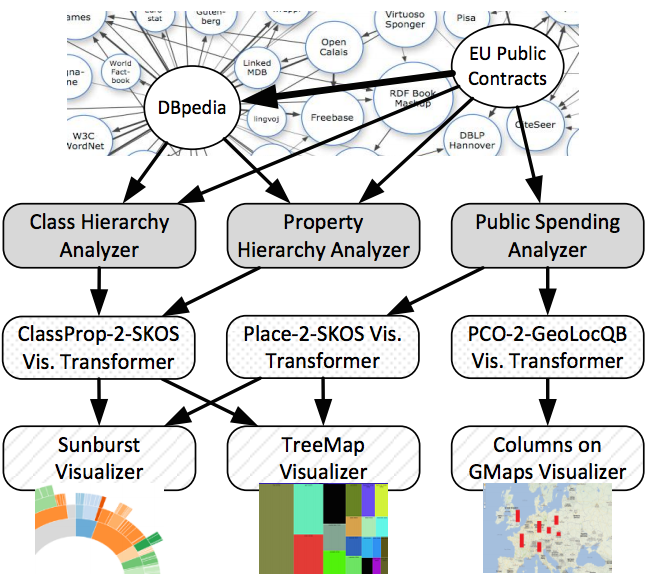
\includegraphics[scale=0.8]{img/ldvm-lod.png}
\label{fig:ldvm-lod}
\caption{Sample application of analyzers and visualizers in a LDVM pipeline.}
\end{figure}

\section{Visualization Applications Over Linked Data}
\label{sec:visAppsLD}

As many initiatives on Linked Open Data is growing, tools and technologies are getting more and more mature to help pro-consumers to leverage the lifting process of the data. At the same times, standardization bodies such as W3C are helping in providing best practices to publish Open Government Data by using appropriate vocabularies, taking care of stability in the URIs policies, and making links to other datasets. It is the case for example of the Government Linked Data Working Group\footnote{\url{http://www.w3.org/2011/gld/}} which is developing standards to help governments publishing their data using Semantic Web technologies. Having a look at different proposals of the Life Cycle of Government LD, one of the last stage is ``Publication'' where the data is released according to the 4-5 stars principles\footnote{\url{http://5stardata.info/}}, with a given access to a SPARQL endpoint. However, for a better understanding of the data, one of the next step is usually to building visualizations through intuitive charts, graphs , etc. that will benefit to citizens, data journalists and other public authorities to improve the quality of their decisions. At the moment, one way of doing is to look around previous initiatives to see what type of application is already there, and make something similar according to a given dataset. Another approach is by organizing \textit{contests} where the challenges are to mash up unexpected datasets with clear and beautiful visualizations. Such approach is harder as developers also try figure out which tool and library is used for different applications. What if we describe applications according to the facets/views, datasets, visual tools etc.? 
%In this paper, we propose a small vocabulary aiming at describing applications developed on top of LOD for more interoperability and components reusability. 
%This paper is organized as follow: Section \ref{sec:apps} defines the types of applications on LOD, followed by a framework for assessing tools for building such applications (cf. Section \ref{sec:frame}). Section \ref{sec:reusable} deals with the facts which are common to many visual applications, and Section \ref{sec:dvia} presents the vocabulary for describing the semantics of mashups. We make some references to similar works in Section \ref{sec:rworks} and provide some outlook in Section 

\section{Catalog of Applications on the Web} \label{sec:rworks}
% Mention the efforts of UNiv Southampton for describing the apps developed cfr http://data.southampton.ac.uk/dumps/apps/2012-12-18/apps.ttl
% Mention the efforts at RPI for some of the apps developed for data.gov.
\textcolor{red}{re-read paper approaches to visualising Linked Data: A survey (Aba-Sah and M. Rowe)} \\

The Open Data Service at the University of Southampton\footnote{\url{http://data.southampton.ac.uk/apps.htm}} has a register of all the applications developped using their datasets. A catalog of the Applications using the data is available at \url{http://id.southampton.ac.uk/dataset/apps}. Each application is described by giving the name, the type of the application, date of creation, the creator and the datasets used. There is also a flag to specify if the application is ``official'' or not. This initiative seems to be isolated and by having a common layer of vocabulary for the applications, we could add more informations as it is intended in DVIA vocabulary. 

Another approach at Rensseler Institute\footnote{\url{http://data-gov.tw.rpi.edu}} is to put at the bottom of the static page of the demo/application showcasing the benefits of Open Data for data.gov. is to put information, containing also a link to the SPAQRL query used for generating the application. As this information is human-readable and can help, the main drawback is the lack of a machine-readable version, using semantics. DVIA can leverage the issue aggregating many such descriptions in other Open Data initiatives as well. 

Regarding the tools for visualizing Linked Data,  the paper \cite{aba2011} analyses in detail the current approaches used to browse and visualize Linked Data, by identifying requirements for users classify into two groups: tech-savvy and lay-users. As the authors extensively surveyed more generic Linked Data browsers, with text-based presentation and visualization options, they provide some recommendations according to the size of the data such as fine-grained analysis among others. However, they do not target their study on tools that can easily help building visual Semantic Web-based applications. However, our approach is to study the tools used to build innovative applications for detecting the components that could be reusable across different domain y/o scope. 

\section{Linked Data Applications} \label{sec:apps}
According to \cite{card99}, \texttt{Visualization} is \textit{ ``the use of computer-supported, interactive visual representations to amplify cognition''}. So the unique object of visualization is developing insights from collected data. That justify why each time a new dataset is released, users always expected some showcases to play with the underlying datasets. It is true that many public open initiatives uses incentives actions like \textit{challenges}, \textit{datahackday} or \textit{contest}, etc. to find innovative applications that actually exhibit the benefits of datasets published. Visualizations play crucial role as they can easily find errors in a large collection; detect patterns in a dataset or help navigate through the dataset. 

\subsection{Typology of Applications}
Jeni Tennison\footnote{\url{http://www.theodi.org/people/jeni}} defines  in her blog\footnote{\url{http://www.jenitennison.com/blog/node/126}} three categories of applications using online data:
\begin{itemize}
\item (i) \textit{data-specific applications}, which are constructed around particular data sets that are known to the developer of the application; hence the visualizations obtained are of data-specific applications. Examples are the famous applications of ``Where does my money go''  in Greece\footnote{\url{http://publicspending.medialab.ntua.gr/en/index.php}} or UK\footnote{\url{http://wheredoesmymoneygo.org/}}. Those applications are also called ``mashups". 
\item (ii) \textit{vocabulary-specific applications}, which are constructed around particular vocabularies, wherever the data might be found that uses them. Examples here are FaceBook� Social Graph API , IsaViz\footnote{\url{http://www.w3.org/2001/11/IsaViz}}, among others
\item (iii) \textit{generic applications}, which are constructed to navigate through any RDF that they find; e.g.Tabulator\cite{tabulator06}, OpenLink Data Explorer\footnote{\url{http://ode.openlinksw.com/}}

\end{itemize}
Because most mashups are data-specific applications, it is important and necessary to  know what information the dataset contains. This could be achieve by giving the meaning of some properties or classes of the vocabularies used to create the dataset. Hence, what the data publisher needs to do very often is to make sure that the data they publish is documented. However, what is seeing in practice, is to consider using an intuitive visualization self-descriptive to both show the added-value of the data and its documentation.

\subsection{Libraries } \label{sec:frame}



The outcome of this state-of-the-art can then be used to assess in the choice of a given visualization tool, according to some criteria, such as (i) usability, (ii) visualization capabilities, (iii) data accessibility, (iv) deployment and (v) extensibility. For more details on this survey, the readers are encouraged to read \cite{deliverable2012b}.\footnote{Note: The survey does not contain Visual Box as it was not released at the time of writing the survey}. Table \ref{tab:visuTools} gives an overview of the selected tools studied.

\begin{landscape}
\begin{table}[ht]
\centering
\begin{tabularx}{\linewidth}{ |X|X|X|X|X|X|X|X|X|}
\hline
\textbf{Tools} & \textbf{Data Formats}& \textbf{Data Access} & \textbf{Language Code} & \textbf{Type of Views} & \textbf{Imported Libraries} & \textbf{License} & \textbf{SemWeb Compliant} & \textbf{Creator} \\
\hline
Choosel & xls, csv & API & GWT & Text, Map, Bar chart & Time (Simile), Protovis, charts, Flexvis & Open & No & Lars Grammel\\
\hline
Fresnel & RDF & --& RDF& Propertie,  Labels & Welkin, IsaViz, Haystack, CSS &  Open & Yes & Emmanuel Pietriga et al. \\
\hline
Spark & RDF-JSON & SPARQL& PHP& Date chart, Pie chart, simple table &  -- &  Open & Yes & AIFB-KIT \\
\hline
LDA & RDF & SPARQL& Java, PHP& -- &  -- &  Open & Yes & Talis, Epimorphis \\
\hline
Semantic Web Import & RDF & SPARQL CONSTRUCT& Netbeans& Graph Node Views &  -- &  CECILL-B & Yes & Wimmics (INRIA) \\
\hline
Many Eyes & xls, plain text and HTML & API& Java, Flash& charts, trees, graphs, maps & --&  IBM & No & IBM research \\
\hline
D3.js & CSV, SVG, GeoJson & API& JavaScript& charts, trees, graphs, maps & Jquery, sizzle, colorbrewer& Open & Possible & Mike Bostock \\
\hline
Facet Spatial Semantic Browsing Widgets & RDF- JSON & SPARQL& JavaScript& Map,Facet view & Jquery, dynatree&  Open & Yes & AKSW \\
\hline
Sgvizler & RDF- JSON & SPARQL SELECT& JavaScript& Map, Line chart, timeline, sparkline & Google visualization API&  Open & Yes & Martin G. Skjaeland \\
\hline
Visual Box & RDF & SPARQL SELECT& PHP, Django template& Map, charts, timeline, graphs & Google charts, TimeKnots, d3.js&  Open & Yes & Alvaro Graves (RPI) \\
\hline
Map4rdf & RDF- JSON & SPARQL & Java, GWT& Facet, Map & OSM Layers, Google Maps&  Open & Yes & OEG (UPM) \\
\hline
Exhibit & JSON Exhibit & Data dump& JavaScript& Map,Tile, Thumbnail, Tabular and Timeline & ---&  Open & Yes & MIT \\
\hline
Google Visualization API & JSON, CSV & API& JavaScript& Many charts, controls and dashboard & AJAX API&  Open & Possible & Google \\
\hline
Data Publica & DSPL & API& JavaScript& Map,graph, histogram, table & Google charts, highchart.js& Proprietary & No & Data Publica \\
\hline
GeoAPI & GML, KML, GPX & API& JavaScript& Map views & OpenLayers, Prototype.js& Free for non commercial use & Yes & IGN (France) \\
\hline
\end{tabularx}
\caption{Survey of some tools used for creating visualizations on the Web.}
\label{tab:visuTools}
\end{table}
\end{landscape}

\subsection{On Reusable Applications} \label{sec:reusable}
%\todo{ summary of the application survey D6.1: diversity, scope, and countries} 
%\todo{show with the sample of openspending.fr} \\
%\todo{ The choice of the features used}
We first review the numerous applications that have been developed on top of datasets  opened by governments (UK, USA, France) and public local authorities. We made a random survey of thirteen (13) applications \cite{deliverable2012a} in various domains such as of security, health, finance, transportation, housing, city, foreign aid and education. The main template used was to find out:
\begin{itemize}
\item the name of the application:
\item the scope or target domain of the application;
\item a small and concise description;
\item the platform on which the application can be deployed and view;
\item the policy used for creating the URL of the application;
\item the legacy data used to build the application, and a mention of the process of the lifting process of the raw data to RDF if available;
\item the different views available of the application;
\item comments or relevant drawback to mention;
\item the license of the application
\end{itemize}
 Table \ref{tab:describeApps} provides the information extracted from \texttt{openspending in Greece} using the aforementioned template. 


\begin{table}[ht!bp]
    \caption{Gathering reusable information from openspending in Greece Application} \label{tab:describeApps}
    \small
    \center
    \begin{tabularx}{\textwidth}{@{}lX@{}}
     %\begin{tabular}{@{}llX@{}}
    \toprule
    \textbf{Features} & \textbf{Value}\\
    \toprule
    \texttt{Access Url }&	\url{http://publicspending.medialab.ntua.gr/}\\
    \midrule
    \texttt{Scope/Domain} &	Public spending, Government \\
    \midrule
    \texttt{Description} & The application helps visualizing the most characteristic facts of the Greek public spending, interconnected to foreign expenditure and other data. \\
    \midrule
    \texttt{Supported Platform} &	Web \\ 
    \midrule
    \texttt{URL Policy}   &  http://{BASE}/en/{NAME-CHART}.php e.g., \url{http://{BASE}/en/toppayersday.php} \\
    \midrule
    \texttt{Data Source}	& \url{http://opendata.diavgeia.gov.fr}; Greek Tax data (TAXIS) \\ 
    \midrule
\texttt{Type of views} & Bubble tree, column and bar charts \\ 
    \midrule
   \texttt{Visualization tools} &  HighchartsJS,  Bubble TreeJS JqueryJS ; RaphaelJS \\ 
   \midrule
  \texttt{License} & Open \\ 
    \midrule
\texttt{Business Value} & Not Commercial (Free) \\ 
    \bottomrule
  
    % \end{tabular}
    \end{tabularx}
    \end{table}
   
 \section{Evaluating Visualizations}
 See Roberto Garcia work and proposal in Datalift technical report.

  \section{Summary}
  
